\documentclass[serif,10pt,t]{beamer}
\usepackage[ruled, linesnumbered]{algorithm2e}
\usepackage{epsfig, subfigure, amssymb, multirow, algorithmic,amsmath, graphics,rotating,multirow,colortbl,xcolor,graphicx,subfigure}
\usepackage{latexsym,amssymb,epsfig,graphicx,subfigure,rotating,multirow,colortbl,xcolor,amsmath,algorithmic,booktabs}
\usecolortheme[rgb={.31,0.51,0.75}]{structure}
%\usepackage{kbordermatrix}
%\usecolortheme[rgb={0.15,0.55,0.25}]{structure}
%\usecolortheme[rgb={0.35,0.60,0.25}]{structure}
\usetheme{Warsaw}
\newcommand*{\superscript}[1]{\ensuremath{^{\rm #1}}}
\newcommand*{\subscript}[1]{\ensuremath{_{\rm #1}}}

% \beamerdefaultoverlayspecification{<+->}
%\newtheorem{theorem}{Theorem}


%%%%% Set up the coloured tables %%%%%
\colorlet{tableheadcolor}{gray!25} % Table header colour = 25% gray
\colorlet{tablerowcolor}{gray!10} % Table row separator colour = 10% gray
\newcommand{\headcol}{\rowcolor{tableheadcolor}}
\newcommand{\rowcol}{\rowcolor{tablerowcolor}}
\newtheorem{proposition}{Proposition}
\newtheorem{conjecture}{Conjecture}
\newtheorem{observation}{Observation}
\newtheorem{suggestion}{Suggestion}
\newtheorem{question}{Question}
\newtheorem{decision}{Decision}

% The top-most line of a table
\newcommand{\topline}{\arrayrulecolor{black}\specialrule{0.1em}{\abovetopsep}{0pt}%
	\arrayrulecolor{tableheadcolor}\specialrule{\belowrulesep}{0pt}{0pt}%
	\arrayrulecolor{black}}

	% The top-most line of a table
\newcommand{\toplinee}{\arrayrulecolor{black}\specialrule{0.1em}{\abovetopsep}{0pt}%
	\arrayrulecolor{tablerowcolor}\specialrule{\belowrulesep}{0pt}{0pt}%
	\arrayrulecolor{black}}

% The line between the headings and the table body
\newcommand{\midline}{\arrayrulecolor{tableheadcolor}\specialrule{\aboverulesep}{0pt}{0pt}%
	\arrayrulecolor{black}\specialrule{\lightrulewidth}{0pt}{0pt}%
	\arrayrulecolor{white}\specialrule{\belowrulesep}{0pt}{0pt}%
	\arrayrulecolor{black}}

% A line for when the upper row is rowcolor and the next line is white
\newcommand{\midlinecbw}{\arrayrulecolor{tablerowcolor}\specialrule{\aboverulesep}{0pt}{0pt}%
	\arrayrulecolor{black}\specialrule{\lightrulewidth}{0pt}{0pt}%
 	\arrayrulecolor{white}\specialrule{\belowrulesep}{0pt}{0pt}%
	\arrayrulecolor{black}}

% A line with no black, to further separate a rowcolor row and a white row
\newcommand{\midlinecw}{\arrayrulecolor{tablerowcolor}\specialrule{\aboverulesep}{0pt}{0pt}%
	\arrayrulecolor{tablerowcolor}\specialrule{\lightrulewidth}{0pt}{0pt}%
	\arrayrulecolor{white}\specialrule{\belowrulesep}{0pt}{0pt}%
	\arrayrulecolor{black}}

% A line for when the upper row is white and the next line is rowcolor
\newcommand{\midlinewbc}{\arrayrulecolor{white}\specialrule{\aboverulesep}{0pt}{0pt}%
	\arrayrulecolor{black}\specialrule{\lightrulewidth}{0pt}{0pt}%
	\arrayrulecolor{tablerowcolor}\specialrule{\belowrulesep}{0pt}{0pt}%
	\arrayrulecolor{black}}

% sadfsdfsdf sdfsdfsdf
\newcommand{\midlinehr}{\arrayrulecolor{white}\specialrule{\aboverulesep}{0pt}{0pt}%
	\arrayrulecolor{black}\specialrule{\lightrulewidth}{0pt}{0pt}%
	\arrayrulecolor{tableheadcolor}\specialrule{\belowrulesep}{0pt}{0pt}%
	\arrayrulecolor{tablerowcolor}}


% A line for the bottom of the table, when the last row is white
\newcommand{\bottomline}{\arrayrulecolor{white}\specialrule{\aboverulesep}{0pt}{0pt}%
	\arrayrulecolor{black}\specialrule{\heavyrulewidth}{0pt}{\belowbottomsep}}%

% A line for the bottom of the table, when the last row is rowcolor
\newcommand{\bottomlinec}{\arrayrulecolor{tablerowcolor}\specialrule{\aboverulesep}{0pt}{0pt}%
	\arrayrulecolor{black}\specialrule{\heavyrulewidth}{0pt}{\belowbottomsep}}%

\newcommand{\bottomlinect}{\arrayrulecolor{tableheadcolor}\specialrule{\aboverulesep}{0pt}{0pt}%
	\arrayrulecolor{black}\specialrule{\heavyrulewidth}{0pt}{\belowbottomsep}}%
%%%%% Set up the coloured tables %%%%%

% sadfsdfsdf sdfsdfsdf
\newcommand{\midlinewbh}{\arrayrulecolor{white}\specialrule{\aboverulesep}{0pt}{0pt}%
	\arrayrulecolor{black}\specialrule{\lightrulewidth}{0pt}{0pt}%
	\arrayrulecolor{tableheadcolor}\specialrule{\belowrulesep}{0pt}{0pt}%
	\arrayrulecolor{tableheadcolor}}

\newcommand{\midlinecbh}{\arrayrulecolor{tablerowcolor}\specialrule{\aboverulesep}{0pt}{0pt}%
	\arrayrulecolor{black}\specialrule{\lightrulewidth}{0pt}{0pt}%
	\arrayrulecolor{tableheadcolor}\specialrule{\belowrulesep}{0pt}{0pt}%
	\arrayrulecolor{tableheadcolor}}


\begin{document}
\title[{QSS Solver and LIQSS2 \hspace{0.4cm} \insertframenumber/\inserttotalframenumber}]{{\sc QSS Solver and LIQSS2}}
\author[AP de Villiers]{{AP de Villiers} \newline \newline \footnotesize 30 May 2016}
\date{}
%\institute{}

\begin{frame}
\begin{center}
\vspace{0.1cm}

\includegraphics[scale=1]{HQLogo.png}
\end{center}
\titlepage
\end{frame}




\begin{frame}\frametitle{QSS Solver Stats}
\begin{itemize}
\item Some stats
\begin{itemize}
\item 891 documents in total
\item 59 C files
\item 79 Cpp files
\item 142 header files
\item Many makefiles, scripting file extentions and .so library files as well
\end{itemize}
\item SVN Repo creation date: 2012-03-18
\item QSS Solver version 3.1
\item 114 MB in size
\item Active commits on repo
\end{itemize}

\end{frame}


\begin{frame}\frametitle{Why we emulate QSS Solver?}
 \begin{itemize}
  \item We want to incorporate the LIQSS method into OpenModelica
  \item The QSS literature does not provide enough algorithmic details
  \item We can use the code of QSS Solver to understand the in-depth detail of LIQSS methods
  \item We gain access to additional info that we require related to specific models
  \item We can use the research to write a LIQSS2 solver in OpenModelica.
 \end{itemize}
\end{frame}

\begin{frame}\frametitle{Why is this not a simple process?}
 The main reasons include the following:
 \begin{itemize}
  \item No comments are present in QSS Solver
  \item Variable abbreviations are often used
  \item Most of the procedures in the code are not explained/described in the QSS literature at all.
  \item The templating section of code has not been studied at all.
  \item Function pointers make it difficult to resolve actual function calls.
 \end{itemize}
\end{frame}

\begin{frame}\frametitle{What we have done to date}
 \begin{itemize}
  \item LIQSS2 in OpenModelica (Lotka-Volterra)
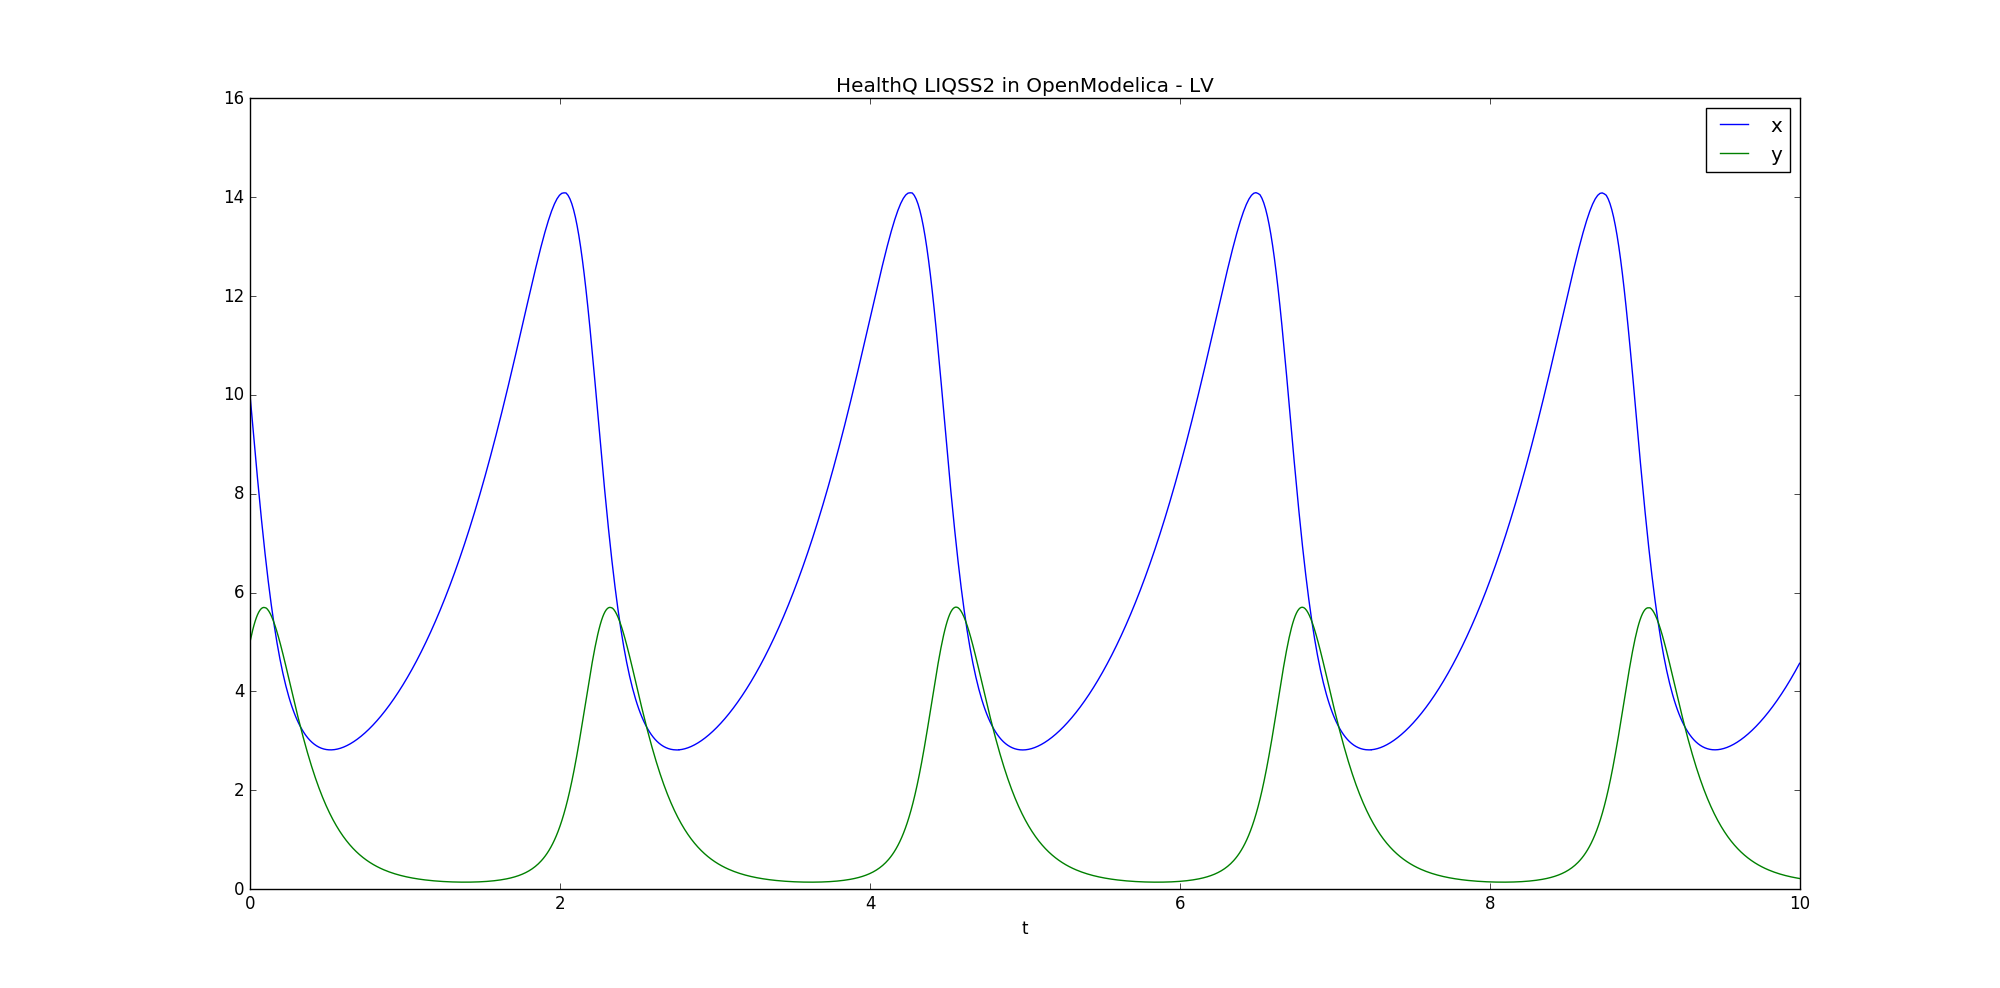
\includegraphics[scale=0.21]{1-LV.png}

 \end{itemize}

\end{frame}



\begin{frame}\frametitle{What we have done to date}
 \begin{itemize}
  \item LIQSS2 in OpenModelica  with simple events (Lotka-Volterra)
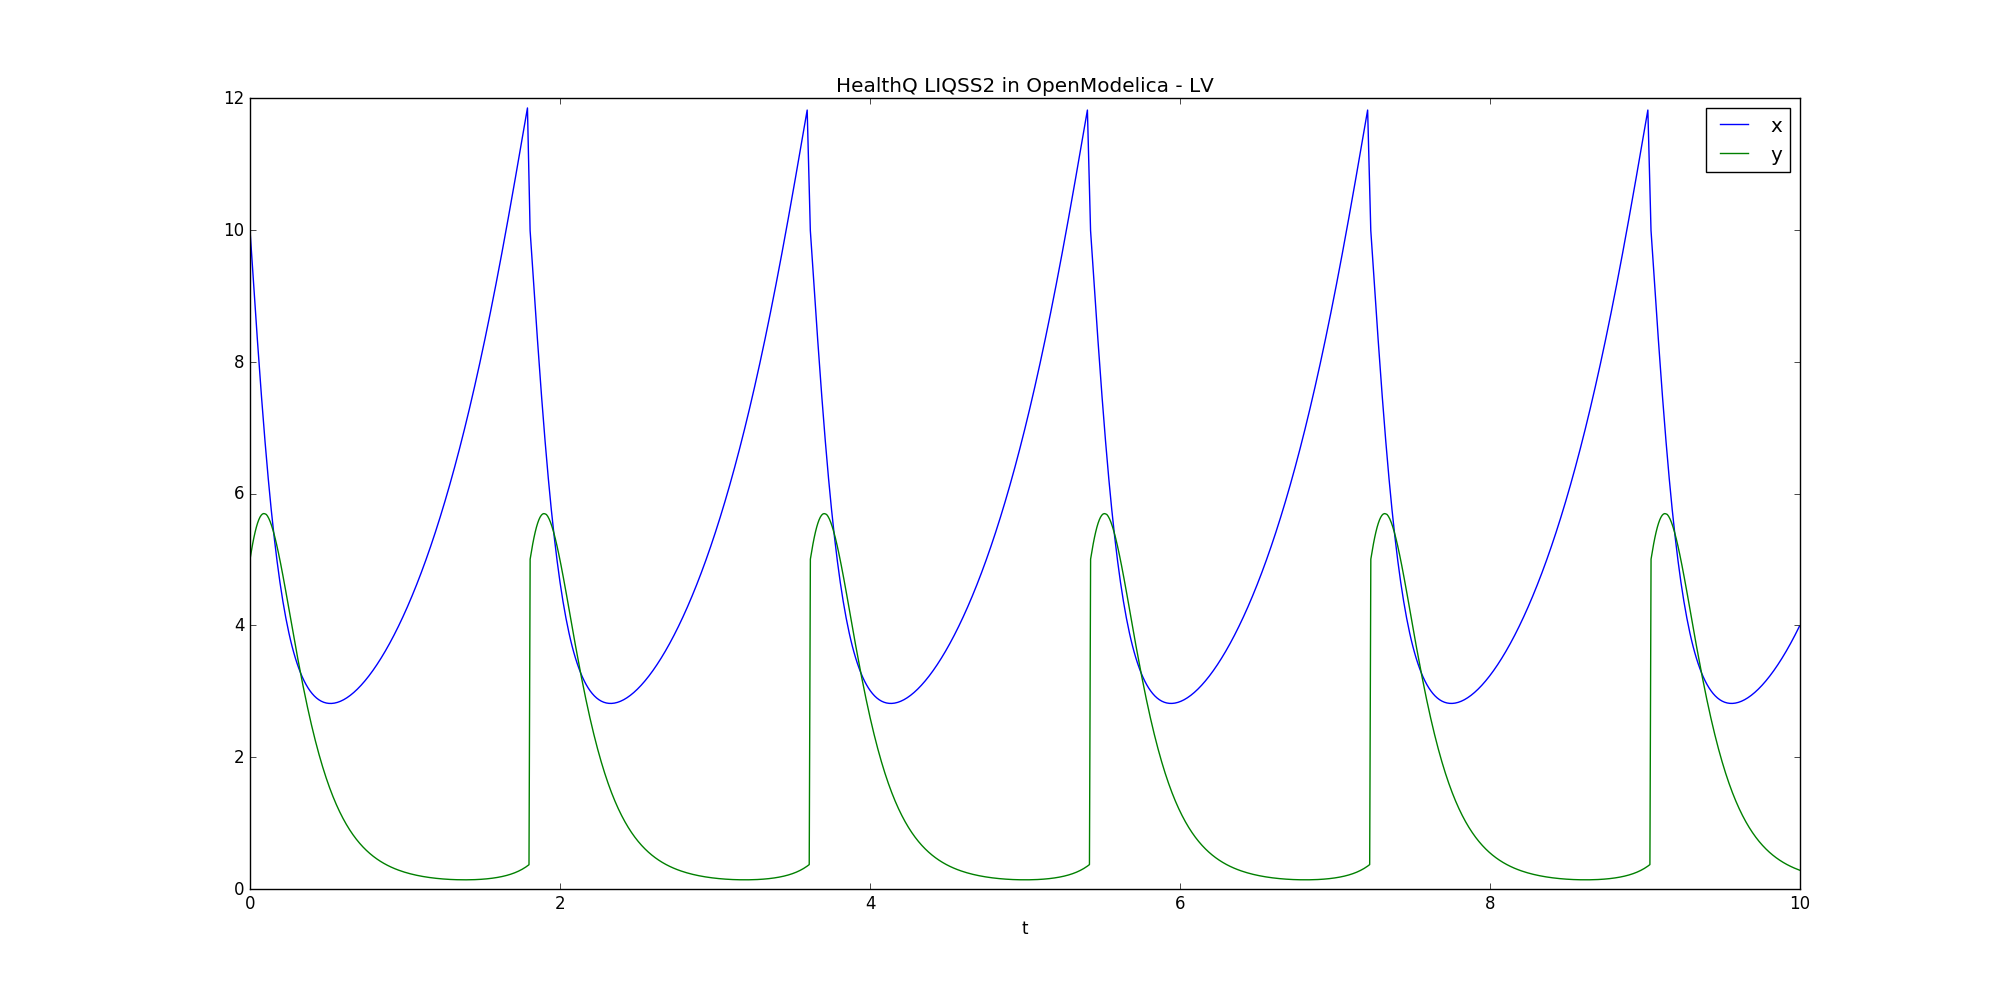
\includegraphics[scale=0.21]{2-LV.png}

 \end{itemize}

\end{frame}


\begin{frame}\frametitle{Comparing these results}
 \begin{itemize}
  \item For this Lotka-Volterra model, there is very little difference between the model with events and the one without events, as the state variables are all merely reinitialized during the event.
  \item The simulation thus restarts the simulation in the same manner during each simulation.
  \item No root finding was done in the code for this kind of event in QSS Solver.
  \item The timing of when state variables must be updated is simple, since  we have a simple model.
 \end{itemize}

\end{frame}



\begin{frame}\frametitle{Moving on to more detailed models}
 \begin{itemize}
  \item We looked at the bouncing ball example
  \item In our model the bouncing of the ball is irregular.
  \item We then looked at how QSS Solver addresses the model.
  \item Some interesting things were noticed:
  \begin{itemize}
   \item The model created a .c file with many more variables created than in the Lotka-Volterra model.
   \item Limited understanding of these variables and there importance.
   \item The iterative algorithmic implementation has changed -- a different algorithm is used.
  \end{itemize}
  \item Graph based operations found:
  \begin{itemize}
   \item In the Bouncing ball example, the update times of the state variables may abruptly change according to a function ``SC\_update''.
   \item This function often does not influence the outcome of the simulation, but it has an effect.
   \item This function makes use of a graph based structure to recompute the update times.
   \item This is not a trivial function --- it contains many operations and calculations.
   \item The reason for the usage of this function is unclear.
  \end{itemize}


 \end{itemize}

\end{frame}









 \begin{frame}\frametitle{Challenges}
\begin{itemize}
 \item We go into the code of QSS Solver and find the sections of code where our model(s) have an effect.
 \item The reasoning and meaning needs to be deciphered --- we need to understand the math and implementation considerations.
 \item We need to map the method into OpenModelica's framework.
 \item We need to make sure we get the same simulation results as QSS Solver in OpenModelica.
\end{itemize}

 \end{frame}





\begin{frame}\frametitle{Findings}
 \begin{itemize}
  \item The variables (number of variables) created in the .c file change according to the model in the .mo file.
  \item The iterative algorithmic implementation changes according to how the model is dissected.
  \item Events are incorporated in the .c file from the .mo file.
  \item The reasoning behind many of the variables are still unclear.
  \item The operations of certain functions and their impact are not clear and have not been explored.
 \end{itemize}

 \vspace{.5cm}
  \begin{itemize}
\item General:
 \begin{itemize}
  \item The info of LIQSS in the literature is vastly different from the implementation in QSS Solver.
  \item The reason for the existence of QSS Solver is becoming clear. This answers our question of why LIQSS solvers have not been implemented in OpenModelica.
  \item QSS Solver is a big body of work and requires time to work through.
 \end{itemize}
 \end{itemize}

\end{frame}



\begin{frame}\frametitle{Other considerations}
\begin{itemize}
 \item Symbolic differentiation of second order derivatives --- Martin
 \item Event handling
 \item Understanding/establishing what can be ignored (for now)
\end{itemize}


\end{frame}






\end{document}